% vim: set spell spelllang=en tw=100 et sw=4 sts=4 foldmethod=marker foldmarker={{{,}}} :

\documentclass{beamer}

\usepackage{tikz}
\usepackage{xcolor}
\usepackage{complexity}
\usepackage{hyperref}
\usepackage{microtype}
\usepackage{amsmath}                   % \operatorname
\usepackage{amsfonts}                  % \mathcal
\usepackage{amssymb}                   % \nexists
\usepackage[vlined]{algorithm2e} % algorithms
\usepackage{centernot}
\usepackage{listings}
\usepackage{csquotes}
\usepackage{fancyvrb}
\usepackage{bussproofs}
\usepackage{multicol}
\usepackage{booktabs}
\usepackage{mathtools}
\usepackage{pifont}
\usepackage{marvosym}
\usepackage{cancel}

\RequirePackage[tt=false, type1=true]{libertine}
\RequirePackage[varqu]{zi4}
\RequirePackage[libertine]{newtxmath}
\RequirePackage[T1]{fontenc}

\usetikzlibrary{shapes, arrows, shadows, calc, positioning, fit}
\usetikzlibrary{decorations.pathreplacing, decorations.pathmorphing, shapes.misc}
\usetikzlibrary{tikzmark, backgrounds}
\usetikzlibrary{trees, overlay-beamer-styles}

\definecolor{uofguniversityblue}{rgb}{0, 0.219608, 0.396078}
\definecolor{uofgheather}{rgb}{0.356863, 0.32549, 0.490196}
\definecolor{uofgaquamarine}{rgb}{0.603922, 0.72549, 0.678431}
\definecolor{uofgslate}{rgb}{0.309804, 0.34902, 0.380392}
\definecolor{uofgrose}{rgb}{0.823529, 0.470588, 0.709804}
\definecolor{uofgmocha}{rgb}{0.709804, 0.564706, 0.47451}
\definecolor{uofgsandstone}{rgb}{0.321569, 0.278431, 0.231373}
\definecolor{uofgforest}{rgb}{0, 0.2, 0.129412}
\definecolor{uofglawn}{rgb}{0.517647, 0.741176, 0}
\definecolor{uofgcobalt}{rgb}{0, 0.615686, 0.92549}
\definecolor{uofgturquoise}{rgb}{0, 0.709804, 0.819608}
\definecolor{uofgsunshine}{rgb}{1.0, 0.862745, 0.211765}
\definecolor{uofgpumpkin}{rgb}{1.0, 0.72549, 0.282353}
\definecolor{uofgthistle}{rgb}{0.584314, 0.070588, 0.447059}
\definecolor{uofgrust}{rgb}{0.603922, 0.227451, 0.023529}
\definecolor{uofgburgundy}{rgb}{0.490196, 0.133333, 0.223529}
\definecolor{uofgpillarbox}{rgb}{0.701961, 0.047059, 0}
\definecolor{uofglavendar}{rgb}{0.356863, 0.301961, 0.580392}

% {{{ theme things
\useoutertheme[footline=authortitle]{miniframes}
\useinnertheme{rectangles}

\setbeamerfont{block title}{size={}}
\setbeamerfont{title}{size=\large,series=\bfseries}
\setbeamerfont{section title}{size=\large,series=\mdseries}
\setbeamerfont{author}{size=\normalsize,series=\mdseries}
\setbeamercolor*{structure}{fg=uofguniversityblue}
\setbeamercolor*{palette primary}{use=structure,fg=black,bg=white}
\setbeamercolor*{palette secondary}{use=structure,fg=white,bg=uofgcobalt}
\setbeamercolor*{palette tertiary}{use=structure,fg=white,bg=uofguniversityblue}
\setbeamercolor*{palette quaternary}{fg=white,bg=black}
\setbeamercolor{block body}{bg=structure!10}
\setbeamercolor{block title}{bg=structure,fg=white}
\setbeamertemplate{blocks}[rounded]
\setbeamercolor*{titlelike}{parent=palette primary}

\beamertemplatenavigationsymbolsempty

\setbeamertemplate{title page}
{
    \begin{tikzpicture}[remember picture, overlay]
        \node at (current page.north west) {
            \begin{tikzpicture}[remember picture, overlay]
                \fill [fill=uofguniversityblue, anchor=north west] (0, 0) rectangle (\paperwidth, -3.0cm);
            \end{tikzpicture}
        };

        \node (logo) [anchor=north east, shift={(-0.6cm,-0.2cm)}] at (current page.north east) {
            \includegraphics[keepaspectratio=true,scale=0.5]{../../images/UoG_keyline.pdf}
        };

        \node (logo2) [anchor=north, below=0.2cm of logo.south] {
            \includegraphics[keepaspectratio=true,scale=0.1]{../../images/RAEngWhite.pdf}
        };

        \coordinate (logos) at ($(logo.south)!0.5!(logo2.north)$);

        \node [anchor=west, xshift=0.2cm] at (current page.west |- logos) {
            \begin{minipage}{0.65\paperwidth}\raggedright
                {\usebeamerfont{title}\usebeamercolor[white]{}\inserttitle}\\[0.2cm]
                {\usebeamerfont{author}\usebeamercolor[white]{}\insertauthor}\\[0.2cm]
                {\usebeamerfont{author}\usebeamercolor[white]{}\tiny With numerous co-conspirators, including Bart Bogaerts, Jan Elffers, \\
                Stephan Gocht, Ross McBride, Matthew McIlree, Jakob Nordstr{\"o}m, \\
                Andy Oertel, Patrick Prosser, and James Trimble \\[0cm]}
            \end{minipage}
        };
    \end{tikzpicture}
}

\setbeamertemplate{section page}
{
    \begin{centering}
        \begin{beamercolorbox}[sep=12pt,center]{part title}
            \usebeamerfont{section title}\insertsection\par
        \end{beamercolorbox}
    \end{centering}
}

\newcommand{\frameofframes}{/}
\newcommand{\setframeofframes}[1]{\renewcommand{\frameofframes}{#1}}

\makeatletter
\setbeamertemplate{footline}
{%
    \begin{beamercolorbox}[colsep=1.5pt]{upper separation line foot}
    \end{beamercolorbox}
    \begin{beamercolorbox}[ht=2.5ex,dp=1.125ex,%
        leftskip=.3cm,rightskip=.3cm plus1fil]{author in head/foot}%
        \leavevmode{\usebeamerfont{author in head/foot}\insertshortauthor}%
        \hfill%
        {\usebeamerfont{institute in head/foot}\usebeamercolor[fg]{institute in head/foot}\insertshortinstitute}%
    \end{beamercolorbox}%
    \begin{beamercolorbox}[ht=2.5ex,dp=1.125ex,%
        leftskip=.3cm,rightskip=.3cm plus1fil]{title in head/foot}%
        {\usebeamerfont{title in head/foot}\insertshorttitle}%
        \hfill%
        {\usebeamerfont{frame number}\usebeamercolor[fg]{frame number}\insertframenumber~\frameofframes~\inserttotalframenumber}
    \end{beamercolorbox}%
    \begin{beamercolorbox}[colsep=1.5pt]{lower separation line foot}
    \end{beamercolorbox}
}

\makeatletter
\newenvironment{nearlyplainframe}[2][]{
    \def\beamer@entrycode{\vspace*{-\headheight}\vspace*{3pt}}
    \setbeamertemplate{headline}
    {%
        \begin{beamercolorbox}[colsep=1.5pt]{upper separation line head}
        \end{beamercolorbox}
        \begin{beamercolorbox}[ht=0.5ex,dp=0.125ex,%
            leftskip=.3cm,rightskip=.3cm plus1fil]{title in head/foot}%
        \end{beamercolorbox}%
        \begin{beamercolorbox}[ht=0.5ex,dp=0.125ex,%
            leftskip=.3cm,rightskip=.3cm plus1fil]{author in head/foot}%
        \end{beamercolorbox}%
        \begin{beamercolorbox}[colsep=1.5pt]{lower separation line head}
        \end{beamercolorbox}
        \vspace*{\headheight}
    }

    \setbeamertemplate{footline}
    {%
        \begin{beamercolorbox}[colsep=1.5pt]{upper separation line foot}
        \end{beamercolorbox}
        \begin{beamercolorbox}[ht=0.5ex,dp=0.125ex,%
            leftskip=.3cm,rightskip=.3cm plus1fil]{author in head/foot}%
        \end{beamercolorbox}%
        \begin{beamercolorbox}[ht=0.5ex,dp=0.125ex,%
            leftskip=.3cm,rightskip=.3cm plus1fil]{title in head/foot}%
        \end{beamercolorbox}%
        \begin{beamercolorbox}[colsep=1.5pt]{lower separation line foot}
        \end{beamercolorbox}
    }

    \begin{frame}[#1]{#2}
    }{
    \end{frame}
}
\makeatother

\makeatletter
\newenvironment{justborderframe}[2][]{
    \def\beamer@entrycode{\vspace*{-\headheight}}
    \setbeamertemplate{headline}
    {%
        \begin{beamercolorbox}[colsep=1.5pt]{upper separation line head}
        \end{beamercolorbox}
        \begin{beamercolorbox}[ht=0.5ex,dp=0.125ex,%
            leftskip=.3cm,rightskip=.3cm plus1fil]{title in head/foot}%
        \end{beamercolorbox}%
        \begin{beamercolorbox}[ht=0.5ex,dp=0.125ex,%
            leftskip=.3cm,rightskip=.3cm plus1fil]{author in head/foot}%
        \end{beamercolorbox}%
        \begin{beamercolorbox}[colsep=1.5pt]{lower separation line head}
        \end{beamercolorbox}
        \vspace*{\headheight}
    }

    \setbeamertemplate{footline}
    {%
        \begin{beamercolorbox}[colsep=1.5pt]{upper separation line foot}
        \end{beamercolorbox}
        \begin{beamercolorbox}[ht=0.5ex,dp=0.125ex,%
            leftskip=.3cm,rightskip=.3cm plus1fil]{author in head/foot}%
        \end{beamercolorbox}%
        \begin{beamercolorbox}[ht=0.5ex,dp=0.125ex,%
            leftskip=.3cm,rightskip=.3cm plus1fil]{title in head/foot}%
        \end{beamercolorbox}%
        \begin{beamercolorbox}[colsep=1.5pt]{lower separation line foot}
        \end{beamercolorbox}
    }

    \begin{frame}[#1]{}
    }{
    \end{frame}
}
\makeatother

\makeatletter
\setbeamertemplate{mini frame}
{%
  \begin{pgfpicture}{0pt}{0pt}{.04cm}{.04cm}
    \pgfpathcircle{\pgfpoint{0.04cm}{0.04cm}}{0.04cm}
    \pgfusepath{fill,stroke}
  \end{pgfpicture}%
}
\setbeamertemplate{mini frame in current subsection}
{%
  \begin{pgfpicture}{0pt}{0pt}{.04cm}{.04cm}
    \pgfpathcircle{\pgfpoint{0.04cm}{0.04cm}}{0.04cm}
    \pgfsetfillcolor{section in head/foot.bg}
    \pgfusepath{fill,stroke}
  \end{pgfpicture}%
}

\setbeamersize{mini frame size=0.10cm, mini frame offset=0.06cm}
\makeatother

\newcommand{\notedge}{\not\sim}
\newcommand*{\rom}[1]{\emph{\romannumeral #1 \relax}}
\newcommand{\neighbourhood}{\operatorname{N}}
\newcommand{\vertexset}{\operatorname{V}}
\newcommand{\degree}{\operatorname{deg}}

\newcommand{\Z}{\mathbb{Z}}
\newcommand{\N}{\mathbb{N}}
\newcommand{\Nplus}{\mathbb{N}^{+}}
\newcommand{\Nzero}{\mathbb{N}_{0}}
\newcommand{\varx}{\ensuremath{x}}
\newcommand{\vara}{a}
\newcommand{\varb}{b}
\newcommand{\olnot}[1]{\overline{#1}}
\newcommand{\derivruleformat}[1]{\textcolor{uofgcobalt}{\textbf{#1}}\xspace}
\newcommand{\langstd}{\ensuremath{L}}
\newcommand{\emptycl}{\bot}
\providecommand{\cdclwidthfirstcol}{0.38\textwidth}
\providecommand{\cdclwidthsecondcol}{0.60\textwidth}
\providecommand{\cdclformulaleftadjust}{\hspace{-1.5mm}}
\providecommand{\landwsp}{\,\land\,}
\newcommand{\coeffa}{a}
\newcommand{\coeffb}{b}
\newcommand{\coeffc}{c}
\newcommand{\coeffd}{d}
\newcommand{\coeffk}{k}
\newcommand{\coeffw}{w}
\newcommand{\consta}{A}
\newcommand{\constb}{B}
\newcommand{\constk}{k}
\newcommand{\constw}{W}
\newcommand{\litell}{\ell}
\newcommand{\factor}{c}
\newcommand{\monomm}{m}
\newcommand{\degd}{d}
\newcommand{\lita}{\ensuremath{a}}
\newcommand{\litb}{\ensuremath{b}}
\newcommand{\litc}{\ensuremath{c}}
\newcommand{\litd}{\ensuremath{d}}
\newcommand{\litl}{\ensuremath{\ell}}
\newcommand{\formf}{F}
\newcommand{\constrc}{C}
\newcommand{\clc}{\ensuremath{C}}
\newcommand{\wrt}{with respect to\xspace}
\newcommand{\objf}{f}
\newcommand{\tvastd}{{\ensuremath{\alpha}}}

\newcommand{\pbdeg}[1]{\numfuncformat{deg}(#1)}

\newcommand{\pbrelation}{\bowtie}

\newcommand{\Lor}{\bigvee}
\newcommand{\Land}{\bigwedge}

\newcommand{\pbconstra}{\textstyle \sum_i \coeffa_i \litell_i \geq \consta}
\newcommand{\pbconstrb}{\textstyle \sum_i \coeffb_i \litell_i \geq \constb}
% Use \pbconstrlincomb with arguments i, a, A, b, B c_a c_b
\newcommand{\pbconstrlincomb}[7]%
    {\textstyle \sum_{#1}
      ({#6} {#2}_{#1} + {#7}{#4}_{#1}) \litell_{#1} 
      \geq
      {#6} {#3} + {#7}{#5}}

\newcommand{\colorblue}[1]{\textcolor{uofgcobalt}{#1}}
\newcommand{\colorred}[1]{\textcolor{uofgpillarbox}{#1}}
\newcommand{\colorgreen}[1]{\textcolor{uofglawn}{#1}}

\newcommand{\limpl}{\rightarrow}
\newcommand{\lequiv}{\leftrightarrow}
\renewcommand{\lequiv}{\,\Leftrightarrow\,}
\newcommand{\lortight}{\!\lor\!}
\newcommand{\set}[1]{\{ #1 \}}
\newcommand{\setsize}[1]{{\left|#1\right|}}

\newcommand\veripbid[1]{\textcolor{uofglavendar}{#1}}
\newcommand\veripbConstraint[1]{\textcolor{uofgcobalt}{#1}}

\newcommand<>{\propfalse}[1]{{\alt#2{\textcolor{uofgpillarbox}{\cancel{#1}}}{#1}}}
\newcommand<>{\propfalsenox}[1]{{\alt#2{\textcolor{uofgpillarbox}{#1}}{#1}}}
\newcommand<>{\proptrue}[1]{{\color#2{uofgcobalt}#1}}

% }}}

\author{Ciaran McCreesh}
\title{Auditable Constraint Programming}

\begin{document}

{
    \usebackgroundtemplate{
        \tikz[overlay, remember picture]
        \node[at=(current page.south), anchor=south, inner sep=0pt]{\includegraphics[keepaspectratio=true, height=\paperheight]{../../images/background.jpg}};
    }
    \begin{frame}[plain,noframenumbering]
        \titlepage
    \end{frame}
}

\section{Solvers}

\begin{frame}{Constraint Solvers are Awesome}
\end{frame}

\begin{frame}{The Slide That Gets Me Into Trouble}
\end{frame}

\section{Proof Logging for SAT}

\begin{frame}{Proof Logging}
        \vspace*{-1em}
        \begin{center}
        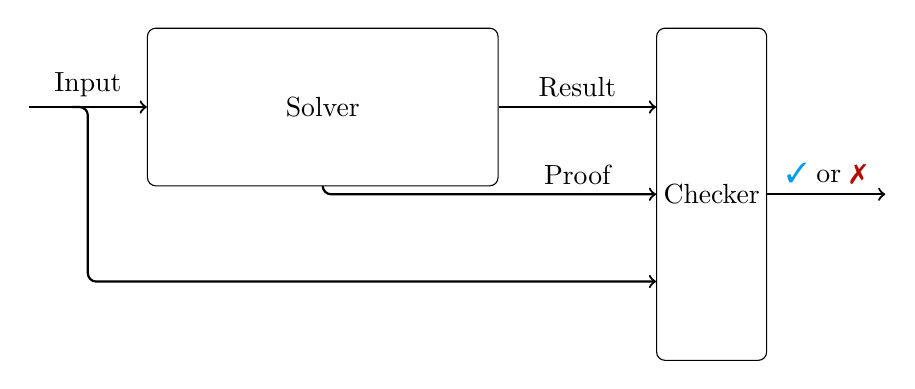
\begin{tikzpicture}
            \node (solver) [%
            inner xsep=5em,
            inner ysep=2.5em, 
            draw, rounded corners=3pt] { Solver };

            \node (checker) [%
            right=2cm of solver.north east, 
            anchor=north west,
            inner xsep=0.25em,
            draw, rounded corners=3pt, 
            minimum height=12em,
            visible on=<3->] { Checker };

            \draw [->, thick] (solver.east) -- (solver.east -| checker.west)
                coordinate [midway] (solutionmid) node [above, midway]
                { Result };

            \draw [->, thick, rounded corners=3pt, visible on=<2->] (solver.south) -- (solver.south |- checker.west)
                -- (checker.west) coordinate [midway] (proofmid);

            \coordinate (prooflabel) at (proofmid-|solutionmid);
            \node [above=0cm of prooflabel, visible on=<2->] { Proof };

            \coordinate [right=1.5cm of checker.east] (verified);
            \draw [->, thick, visible on=<4->] (checker.east) -- (verified) node [above, midway] {
                \textcolor{uofgcobalt}{\ding{51}} or \textcolor{uofgpillarbox}{\ding{55}} };

            \coordinate [left=1.5cm of solver.west] (input);
            \draw [->, thick] (input) -- (solver.west) coordinate [midway] (inputmid) node [above, midway] { Input };

            \coordinate (checkerbotleft) at ($(checker.west)+($(checker.west)-(solver.east-|checker.west)$)$);

            \draw [->, thick, rounded corners=3pt, visible on=<3->] ($(inputmid)+(-0.2,0)$) -- (inputmid) -- (inputmid |- checkerbotleft) -- (checkerbotleft);
        \end{tikzpicture}
      \end{center}

      \vspace{-10mm}

  \begin{enumerate}
  \item<1->
    Run solver on problem input.
  \item<2->
    Get as output not only 
    result   %%%   solution   % -JN
    but also proof.
  \item<3->
    Feed input + 
    result   %%%   solution 
    + proof to proof checker.
  \item<4->
    Verify that proof checker says 
    result   %%%   solution 
    is     correct.
  \end{enumerate}
\end{frame}

\begin{frame}{What Is A Proof?}
    \begin{center}
        \includegraphics[keepaspectratio=true,scale=0.30]{shortest-math-paper.jpg}
    \end{center}
\end{frame}

\providecommand{\litell}{\ell}
\providecommand{\clwidth}{k}

\begin{frame}
  \frametitle{The SAT Problem}

  \vspace{-1mm}
  
  \begin{itemize}
  \item
      \textcolor{uofgcobalt}{Variable} $\varx$: 
    takes value 
%       $1$ (\textbf{true})
    \textbf{true} ($=\!1$)
    or 
%       $0$ (\textbf{false})
    \textbf{false} ($=\!0$)

    \medskip

  \item
      \textcolor{uofgcobalt}{Literal} 
%       $\lita$:  
    $\litell$:  
    variable 
    $\varx$ or its negation
    $\olnot{\varx}$ 
%       (%which we will 
%       %from now on 
%       write
%       $\olnot{\varx}$ 
%       instead of
%       $\lnot{\varx}$)
    

    \medskip
    
  \item
      \textcolor{uofgcobalt}{Clause}
    $\clc = \litell_1 \lor \cdots \lor \litell_{\clwidth}$:
    disjunction of literals \\
    (Consider 
%    clauses 
    as sets, so
    no repetitions and order 
%        is
    irrelevant)
    
    \medskip
    
  \item
      \textcolor{uofgcobalt}{%
      Conjunctive normal form (CNF)
%         CNF 
      formula}
    $\formf = \clc_1 \land \cdots \land \clc_m$:
    conjunction of clauses         
    
%        \bigskip
%        
%      \item
%        \propfalse{\kcnfform{}}:  
%        CNF formula with clauses of size $\leq \clwidth$ \\
%        (assume $\clwidth$ fixed)    
%    
%        \bigskip
%        
%      \item
%        Refer to clauses of \cnfform as
%        \introduceterm{axioms} \\
%        (as opposed to derived clauses)
%    
  \end{itemize}
      

%     \pause
%     \bigskip
  \medskip
  
  \begin{block}{The SAT Problem}
    Given a CNF formula~$\formf$, is it satisfiable?
  \end{block}

%     \pause
%     \bigskip
  \medskip
  
  For instance, what about:
  \begingroup
  \small
  \begin{gather*}
%       &
    ( p \lor \overline{u} )
    \land 
    ( q \lor r )
    \land 
    ( \overline{r} \lor w )
    \land
    ( u \lor x \lor y )
      \ \land \
    \\
%%%    
%       \land \
%       &
    ( x \lor \overline{y} \lor z )
    \land
    ( \overline{x} \lor z )
    \land 
    ( \overline{y} \lor \overline{z} )
    \land 
    ( \overline{x} \lor \overline{z} )
    \land
    ( \overline{p} \lor \overline{u} )
  \end{gather*}
  \endgroup
%   
%     For instance, 
%     what about our example formula?
%     \begin{align*}
%       %        F = \ \ \ \ \  
%       &
%       ( x \lor z ) \land
%       ( y \lor \olnot{z} ) \land
%       ( x \lor \olnot{y} \lor u ) \land
%       ( \olnot{y} \lor \olnot{u} ) \\
%       \land \    
%       &( u \lor v ) \land
%       ( \olnot{x} \lor \olnot{v} ) \land
%       ( \olnot{u} \lor w ) \land
%       ( \olnot{x} \lor \olnot{u} \lor \olnot{w} ) 
%     \end{align*}
%   
  
\end{frame}

%%% Local Variables:
%%% mode: latex
%%% TeX-master: "ProofCplxSATsurvey"
%%% End:



\begin{frame}{Proofs for SAT}

    For satisfiable instances: just
%%% THIS IS JUST confusing at this stage... -JN 
%       give (something that propagates to) 
    specify
    a satisfying assignment.
    \\ \medskip
    For unsatisfiability: 
%       a proof is 
    a sequence of clauses (CNF constraints).
    \begin{itemize}
        \item 
          Each clause follows ``obviously'' from everything we know so far.
        \item 
          Final clause is empty, meaning contradiction (written $\bot$).
        \item
          Means original formula must be inconsistent.
    \end{itemize}
\end{frame}

\begin{frame}[t]{What Is Obvious? Unit Propagation}


  \begin{block}{Unit Propagation}
    Clause
    $\clc$
    \colorblue{unit propagates}
    $\litell$ under partial assignment $\rho$
    if
    $\rho$ falsifies all literals in
    $\clc$ except~$\litell$.
  \end{block}

  \pause
  \bigskip

  \textbf{Example:} Unit propagate for
  $\rho = \set{ p \mapsto 0, q\mapsto 0}$ on
%   
%     \vspace{-4mm}
%   
  \begingroup
  \footnotesize
  \begin{equation*}%
    \cdclformulaleftadjust
    ( 
    \propfalse<3->{p} \lor 
    \proptrue<4->{\overline{u}}
    )
    \landwsp 
    ( \propfalse<3->{q}
    \lor
    \proptrue<5->{r} 
    )
    \landwsp 
    (
    \propfalse<5->{\overline{r}}
    \lor 
    \proptrue<6->{w} 
    )
    \landwsp
    ( 
    \propfalse<4->{u}
    \lor x \lor y )
    \landwsp
    ( x \lor \overline{y} \lor z )
    \landwsp 
    ( \overline{x} \lor z )
    \landwsp 
    ( \overline{y} \lor \overline{z} )
    \landwsp 
    ( \overline{x} \lor \overline{z} )
    \landwsp
    ( 
    \proptrue<3->{\overline{p}} 
    \lor
    \proptrue<4->{\overline{u}}
    )
  \end{equation*}
  \endgroup

  \vspace{-2mm}
 
  \begin{itemize}
  \item<4-> 
    $p \lor \overline{u}$ propagates $u \mapsto 0$.

  \item<5-> 
    $q \lor r$ propagates $r \mapsto 1$.

  \item<6-> 
    Then
    $\overline{r} \lor w$ propagates $w \mapsto 1$.

  \item<7-> 
    No further unit propagations.
  \end{itemize}

  \medskip

  \uncover<8->{%
    Proof checker should 
%       be smart enough to 
    know how to
    unit propagate until saturation.
  }

\end{frame}

\begin{frame}[t]%
%     {Forward Checking (DPLL)}
  {Davis-Putman-Logemann-Loveland (DPLL)}

    DPLL:
  Assign variables and propagate;
  backtrack when clause violated.

  \medskip

%%%   
%%% Lots of text... Try to be more concise -JN  
%%%   
%     We could write a ``proof'' of unsatisfiability
%     by writing a step whenever a forward-checker backtracks
%     asserting the negation of the guesses we made. For example,
%     

  ``Proof trace'':
  when backtracking, write negation
  of guesses made. 


%%%%%
%%%%% Changed to an example that is simpler when highlighting is added -JN
%%%%%

  \begingroup
  \footnotesize
  \begin{equation*}%
%%%
%%% FORMULA *WITH* HIGHLIGHTING
%%%
    \cdclformulaleftadjust
    ( 
    \proptrue<5-5>{p}
    \lor 
    \propfalse<4-5>{\overline{u}}
    )
    \landwsp 
    ( 
    q 
    \lor 
    r 
    )
    \landwsp 
    ( 
    \overline{r} 
    \lor
    w 
    )
    \landwsp
    ( 
    \proptrue<4-5>{u} 
    \lor 
    \only<1-8>{\propfalse<2-8>{x}} 
    \only<9->{\proptrue<9-10>{x}} 
    \lor 
    \only<1-5>{\propfalse<3-5>{y}} 
    \only<6->{\proptrue<6-7>{y}} 
    )
    \landwsp
    ( 
    \only<1-8>{\propfalse<2-8>{x}}
    \only<9->{\proptrue<9-10>{x}}  
    \lor 
    \only<1-5>{\proptrue<3-5>{\overline{y}}}
    \only<6->{\propfalse<6-7>{\overline{y}}} 
    \lor 
    \proptrue<7,10>{z} 
    )
    \landwsp 
    ( 
    \only<1-8>{\proptrue<2-8>{\overline{x}}}
    \only<9->{\propfalse<9-10>{\overline{x}}}  
    \lor 
    \proptrue<7,10>{z} 
    )
    \landwsp 
    ( 
    \only<1-5>{\proptrue<3-5>{\overline{y}}}
    \only<6->{\propfalse<6-7>{\overline{y}}} 
    \propfalse<7>{\lor}
    \propfalse<7,10>{\overline{z}}
    )
    \landwsp 
    ( 
    \only<1-8>{\proptrue<2-8>{\overline{x}}}
    \only<9->{\propfalse<9-10>{\overline{x}}}  
    \propfalse<10>{\lor} 
    \propfalse<7,10>{\overline{z}}
    )
    \landwsp
    (
    \propfalse<5-5>{\overline{p}}
    \propfalse<5-5>{\lor} 
    \propfalse<4-5>{\overline{u}}
    )
%%%
%%% FORMULA WITHOUT HIGHLIGHTING
%%%
%       \cdclformulaleftadjust
%       ( p \lor \overline{u} )
%       \landwsp 
%       ( q \lor r )
%       \landwsp 
%       ( \overline{r} \lor w )
%       \landwsp
%       ( u \lor x \lor y )
%       \landwsp
%       ( x \lor \overline{y} \lor z )
%       \landwsp 
%       ( \overline{x} \lor z )
%       \landwsp 
%       ( \overline{y} \lor \overline{z} )
%       \landwsp 
%       ( \overline{x} \lor \overline{z} )
%       \landwsp
%       ( \overline{p} \lor \overline{u} )
  \end{equation*}
  \endgroup
  
  \bigskip
  
  \begin{columns}[T]%
    \begin{column}{0.4\textwidth}
      \begin{enumerate}
      \item <5-> $x \lor y$
      \item <7-> $x \lor \olnot{y}$
      \item <8-> $x$
      \item <10-> $\olnot{x}$
      \item <11-> $\emptycl$
      \end{enumerate}
    \end{column}
    \begin{column}{0.5\textwidth}
%%%
%%% SEARCH TREE *WITH* OVERLAYS FOR HIGHLIGHTING
%%%
      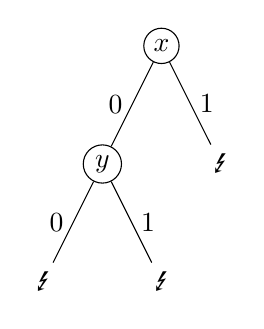
\begin{tikzpicture}<2->%
        [sibling distance=4em, level distance=3.5em, align=center]
        \node [draw, circle, inner sep=2pt, visible on=<2->] {$x$}
        child { node [draw, circle, inner sep=2pt, visible on=<3->] {$y$}
          child { node [visible on=<5->] {\Lightning} edge from parent [visible on=<3->] node [left, visible on=<3->] { 
$0$  %  $\overline{y}$ 
} }
          child { node [visible on=<7->] {\Lightning} edge from parent [visible on=<6->] node [right, visible on=<6->] { 
$1$ % $y$ 
} }
          edge from parent [visible on=<2->] node [left, visible on=<2->] { 
$0$ % $\overline{x}$ 
}
        }
        child { node [visible on=<10->] {\Lightning}
          edge from parent [visible on=<9->] node [right, visible on=<9->] { 
$1$  % $x$
 }
        }
        ;
      \end{tikzpicture}
    \end{column}
  \end{columns}
\end{frame}

\begin{frame}{Reverse Unit Propagation (RUP)}

  To make this a proof, need 
%       each backtrack clause  %%% Trying to fit on one line -JN
  backtrack clauses 
  to be easily verifiable.

  \pause
  
  \begin{block}{Reverse unit propagation (RUP) clause}
    $\clc$ is a 
    \colorblue{reverse unit propagation (RUP)} 
    clause \wrt $\formf$ if
    \begin{itemize}
    \item 
      assigning $\clc$ to false,
    \item 
      then unit propagating on $\formf$ until saturation
    \item 
      leads to contradiction
    \end{itemize}
    If so, 
    $\formf$ clearly  implies  $\clc$,
    and condition easy to verify efficiently
  \end{block}

  \pause
  
  \begin{block}{Fact}
%       Backtracks 
    Backtrack clauses
    from DPLL solver generate a RUP proof.
  \end{block}

\end{frame}

\begin{frame}{RUP Proofs and CDCL}
\begin{block}{Fact}
  All learned clauses generated by CDCL solver are RUP clauses.
\end{block}

\pause
\bigskip

  So short proof of unsatisfiability for
  \begingroup
  \footnotesize
  \begin{equation*}%
    \cdclformulaleftadjust
    (
    \proptrue<11>{p} 
    \lor 
    \proptrue<3-5>{\propfalse<10-11>{\overline{u}}} 
    ) 
    \landwsp
    {( q \lor r )}
    \landwsp
    {( \overline{r} \lor w )}
    \landwsp
    (
    \proptrue<10-11>{\propfalse<3-5>{u}} 
    \lor  
    \proptrue<6-7>{\propfalse<3-5,9-11>{x}} 
    \lor 
    \proptrue<4-5>{y} 
    )
    \landwsp
    ( 
    \proptrue<6-7>{\propfalse<3-5,9-11>{x}} 
    \lor 
    \propfalse<4-5>{\overline{y}} 
    \lor 
    \proptrue<5,7>{z}
    )  
    \landwsp
    (
    \proptrue<3-5,9-11>{\propfalse<6-7>{\overline{x}}}
    \lor
    \proptrue<5,7>{z} 
    )
    \landwsp
    (
    \propfalse<4-5>{\overline{y}} 
    \propfalse<5>{\lor} 
    \propfalse<5,7>{\overline{z}}
    ) 
    \landwsp
    (
    \proptrue<3-5,9-11>{\propfalse<6-7>{\overline{x}}}
    \propfalse<7>{\lor} 
    \propfalse<5,7>{\overline{z}} 
    )
    \landwsp
    (
    \propfalse<11>{\overline{p}} 
    \propfalse<11>{\lor}
    \proptrue<3-5>{\propfalse<10-11>{\overline{u}}} 
    )
  \end{equation*}
  \endgroup
  % 
  is sequence of 
  reverse unit propagation (RUP)
  clauses
  \begin{enumerate}
  \item 
    \propfalsenox<3-5>{$\proptrue<10-11>{u} \lor
      \proptrue<6-7>{\propfalsenox<9-11>{x}}$}
  \item 
    \propfalsenox<6-7>{\proptrue<9-11>{$\olnot{x}$}}
  \item 
      \propfalsenox<8-11>{$\emptycl$}
  \end{enumerate}
\end{frame}

\begin{frame}{Resolution Proofs}
    \begin{block}{Fact}
        RUP proofs can be seen as shorthand for Resolution proofs.
    \end{block}

    \bigskip

    \begin{minipage}[c]{0.25\framewidth}
        \textcolor{uofgcobalt}{\textbf{Model axioms}}
    \end{minipage}\hfill\begin{minipage}[c]{0.70\framewidth}
        \centering From the input
    \end{minipage}\bigskip

    \begin{minipage}[c]{0.25\framewidth}
        \textcolor{uofgcobalt}{\textbf{Resolution}}
    \end{minipage}\hfill\begin{minipage}[c]{0.70\framewidth}\begin{prooftree}
        \AxiomC{$\textcolor{uofglawn}{x_1} \vee \textcolor{uofglawn}{x_2} \vee \ldots \vee
        \textcolor{uofglawn}{x_i} \vee \textcolor{uofgpillarbox}{c}$}
        \AxiomC{$\textcolor{uofgpillarbox}{\overline{c}} \vee \textcolor{uofgcobalt}{y_1} \vee
        \textcolor{uofgcobalt}{y_2} \vee \ldots \textcolor{uofgcobalt}{y_j}$}
        \BinaryInfC{$\textcolor{uofglawn}{x_1} \vee \textcolor{uofglawn}{x_2} \vee \ldots \vee
        \textcolor{uofglawn}{x_i} \vee \textcolor{uofgcobalt}{y_1} \vee
        \textcolor{uofgcobalt}{y_2} \vee \ldots \vee \textcolor{uofgcobalt}{y_j}$}
    \end{prooftree}\end{minipage}

    \bigskip

    \begin{itemize}
        \item To prove unsatisfiability: resolve until you reach the empty clause.
    \end{itemize}
\end{frame}

\section{Beyond SAT}

\begin{frame}{Resolution Can't Count}
    \begin{itemize}
        \item All-different requires exponential length proofs in resolution!
    \end{itemize}
\end{frame}

\begin{frame}{From CNF to Pseudo-Boolean}
    \begin{itemize}
        \item A set of $\{ 0, 1 \}$-valued variables $x_i$, $1$ means true.
        \item Constraints are linear inequalities \[
                \sum_i c_i x_i \ge C
            \]
        \item Write $\overline{x}_i$ to mean $1 - x_i$.
        \item Can rewrite CNF to pseudo-Boolean directly, \begin{align*}
                & x_1 \vee \overline{x}_2 \vee x_3 & \leftrightarrow && x_1 + \overline{x}_2 + x_3 \ge 1
        \end{align*}
    \end{itemize}
\end{frame}

\begin{frame}{Cutting Planes Proofs}
    \begin{minipage}[c]{0.35\framewidth}
        \textcolor{uofgcobalt}{\textbf{Model axioms}}
    \end{minipage}\hfill\begin{minipage}[c]{0.60\framewidth}
        \centering From the input
    \end{minipage}\bigskip

    \begin{minipage}[c]{0.35\framewidth}
        \textcolor{uofgcobalt}{\textbf{Literal axioms}}
    \end{minipage}\hfill\begin{minipage}[c]{0.60\framewidth}\begin{prooftree}
        \AxiomC{~}
        \UnaryInfC{$\ell_i \ge 0$}
    \end{prooftree}\end{minipage}\bigskip

    \begin{minipage}[c]{0.35\framewidth}
        \textcolor{uofgcobalt}{\textbf{Addition}}
    \end{minipage}\hfill\begin{minipage}[c]{0.60\framewidth}\begin{prooftree}
        \AxiomC{$\sum_i a_i \ell_i \ge A$}
        \AxiomC{$\sum_i b_i \ell_i \ge B$}
        \BinaryInfC{$\sum_i (a_i + b_i) \ell_i \ge A + B$}
    \end{prooftree}\end{minipage}\bigskip

    \begin{minipage}[c]{0.35\framewidth}
        \textcolor{uofgcobalt}{\textbf{Multiplication}}\\
        for any $c \in \mathbb{N^+}$
    \end{minipage}\hfill\begin{minipage}[c]{0.60\framewidth}\begin{prooftree}
        \AxiomC{$\sum_i a_i \ell_i \ge A$}
        \UnaryInfC{$\sum_i { c a_i \ell_i } \ge c A$}
    \end{prooftree}\end{minipage}\bigskip

    \begin{minipage}[c]{0.35\framewidth}
        \textcolor{uofgcobalt}{\textbf{Division}}\\
        for any $c \in \mathbb{N^+}$
    \end{minipage}\hfill\begin{minipage}[c]{0.60\framewidth}\begin{prooftree}
        \AxiomC{$\sum_i a_i \ell_i \ge A$}
        \UnaryInfC{$\sum_i {\left\lceil \frac{a_i}{c} \right\rceil} \ell_i \ge \left\lceil \frac{A}{c} \right\rceil$}
    \end{prooftree}\end{minipage}\bigskip
\end{frame}

\begin{frame}{Extension Variables}
  Suppose we want new, fresh variable
  $a$ encoding
  \begin{equation*}
      \textcolor{uofglawn}{
        a 
        \lequiv 
        ( 3x + 2y + z + w \ge 3 )
%           (\varx \land y)
      }
  \end{equation*}

  Introduce constraints
  \begin{equation*}
      \textcolor{uofgcobalt}{
%           a \lor \olnot{\varx} \lor \olnot{y}
%       \qquad
    3 \olnot{a} + 3x + 2y + z + w \ge 3 
%       \olnot{a} \lor \varx
    \qquad
    5 a + 
    3 \olnot{x} + 2 \olnot{y}  + \olnot{z} + \olnot{w} \ge 5
%       \olnot{a} \lor y
}
  \end{equation*}

  Should be fine, so long as $a$ hasn't been used before.
\end{frame}

\begin{frame}{Symmetries}
    \begin{center}
    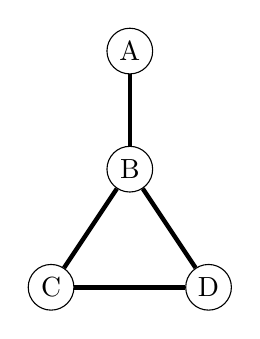
\begin{tikzpicture}
        \node <1> [draw, circle, fill=white, inner sep=4pt, font=\bfseries] (Na) at (1,  0) {\vphantom{1}};
        \node <1> [draw, circle, fill=white, inner sep=4pt, font=\bfseries] (Nb) at (1, -1.5) {\vphantom{1}};
        \node <1> [draw, circle, fill=white, inner sep=4pt, font=\bfseries] (Nc) at (0, -3) {\vphantom{1}};
        \node <1> [draw, circle, fill=white, inner sep=4pt, font=\bfseries] (Nd) at (2, -3) {\vphantom{1}};
        \node at (Na) {A};
        \node at (Nb) {B};
        \node at (Nc) {C};
        \node at (Nd) {D};

        \draw [ultra thick] (Na) -- (Nb);
        \draw [ultra thick] (Nb) -- (Nc);
        \draw [ultra thick] (Nc) -- (Nd);
        \draw [ultra thick] (Nb) -- (Nd);
    \end{tikzpicture}
    \end{center}

    \begin{itemize}
        \item If a solution exists, a solution where $C < D$ exists.
    \end{itemize}
\end{frame}

\begin{frame}{Interleaving RUP and Cutting Planes}
    \begin{itemize}
        \item Can define RUP similarly for pseudo-Boolean constraints.
        \item It does the same thing on clauses.
        \item Idea: use RUP for backtracking, and include explicit cutting
            planes steps to justify reasoning.
    \end{itemize}
\end{frame}

\begin{frame}{The VeriPB System}
    \begin{center}
        \url{https://gitlab.com/MIAOresearch/software/VeriPB} \\
        \bigskip
    \end{center}
    \begin{itemize}
        \item MIT licence, written in Python with parsing in C++.
        \item Useful features like tracing and proof debugging.
    \end{itemize}
\end{frame}

\section{Proof Logging for CP}

\begin{frame}{Making a Proof-Logging Solver}
    \begin{enumerate}
        \item Output a pseudo-Boolean encoding of the problem.
        \item Make the solver log its search tree.
            \begin{itemize}
                \item Output a small header.
                \item Output something on every backtrack.
                \item Output something every time a solution is found.
                \item Output a small footer.
            \end{itemize}
        \item Figure out how to log propagations.
    \end{enumerate}
\end{frame}

\begin{frame}{A Slightly Different Workflow}
    \begin{center}
        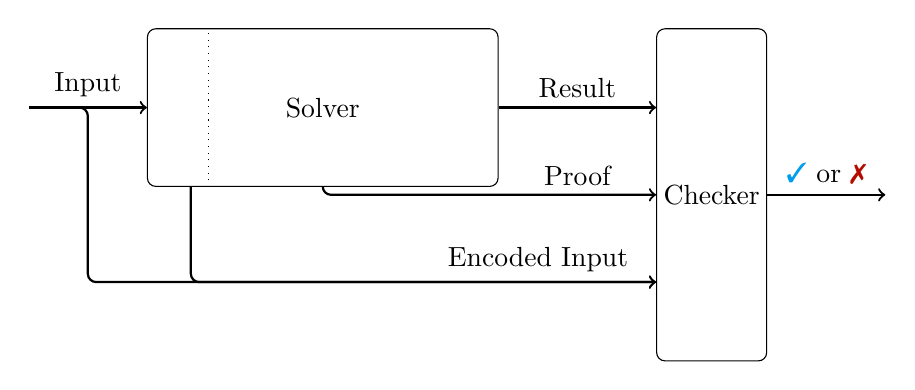
\begin{tikzpicture}
            \node (solver) [inner xsep=5em, inner ysep=2.5em, draw, rounded corners=3pt] { Solver };

            \node (checker) [right=2cm of solver.north east, anchor=north west,
            inner xsep=0.25em, draw, rounded corners=3pt, minimum height=12em, visible on=<3->] { Checker };

            \draw [->, thick] (solver.east) -- (solver.east -| checker.west)
                coordinate [midway] (solutionmid) node [above, midway] { Result };

            \draw [->, thick, rounded corners=3pt, visible on=<2->] (solver.south) -- (solver.south |- checker.west)
                -- (checker.west) coordinate [midway] (proofmid);

            \coordinate (prooflabel) at (proofmid-|solutionmid);
            \node [above=0cm of prooflabel, visible on=<2->] { Proof };

            \coordinate [right=1.5cm of checker.east] (verified);
            \draw [->, thick, visible on=<5->] (checker.east) -- (verified) node [above, midway] {
                \textcolor{uofgcobalt}{\ding{51}} or \colorred{\ding{55}} };

            \coordinate [left=1.5cm of solver.west] (input);
            \draw [->, thick] (input) -- (solver.west) coordinate [midway] (inputmid) node [above, midway] { Input };

            \coordinate (checkerbotleft) at ($(checker.west)+($(checker.west)-(solver.east-|checker.west)$)$);

            \draw [->, thick, rounded corners=3pt, visible on=<3>] ($(inputmid)+(-0.2,0)$) --
            (inputmid) -- (inputmid |- checkerbotleft) -- (checkerbotleft) coordinate [midway] (altinputmid);
            \coordinate (solverstart) at ($(solver.south)!0.75!(solver.south west)$);
            \coordinate (solverstart2) at ($(solver.south)!0.65!(solver.south west)$);
            \draw [dotted, visible on=<4->] (solverstart2) -- (solverstart2 |- solver.north);
            \draw [->, thick, rounded corners=3pt, visible on=<4->] (solverstart) -- (solverstart |- checkerbotleft) -- (checkerbotleft);

            \coordinate (prooflabel) at (altinputmid-|solutionmid);
            \node [above=0cm of prooflabel, xshift=-0.5cm, visible on=<4->] { Encoded Input };
        \end{tikzpicture}
    \end{center}
\end{frame}

\begin{frame}{Encoding Variables}
\end{frame}

\begin{frame}{Encoding Constraints}
\end{frame}

\begin{frame}{Logging Search}
\end{frame}

\begin{frame}{Justifying All-Different}
\end{frame}

\begin{frame}{Progress So Far on World Domination}
    \only<1>{
        \url{https://github.com/ciaranm/glasgow-constraint-solver} \\
        \bigskip
    \begin{itemize}
        \item Absolute value.
        \item All-different.
        \item Circuit (check and prevent).
        \item Element.
        \item Integer linear (in)equalities (with large domains, and GAC
            reformulation).
        \item Minumum and Maximum.
        \item Regular (and hence Stretch, Geost, DiffN).
        \item Smart Table (and hence Lex, At Most One, Not All Equal).
    \end{itemize}}\only<2>{
    \begin{itemize}
        \item SAT with symmetries, cardinality, XOR reasoning, MaxSAT.
            \begin{itemize}
                \item Uncovered several undetected bugs in state of the art solvers.
                \item Can't do MaxSAT hitting set solvers yet, MIP isn't proof logged.
            \end{itemize}
        \item Certified translations from pseudo-Boolean to CNF.
        \item Clique, subgraph isomorphism, maximum common (connected) induced subgraph.
        \item In progress: MIP preprocessing, dynamic programming, \ldots
    \end{itemize}
}
\end{frame}


\section{Challenges}

\begin{frame}{What Reasoning Can We Justify?}
    \begin{itemize}
        \item With extension variables, as strong as Extended Frege.
        \item So according to theorists, we can simulate pretty much everything.
            \begin{itemize}
                \item <2-> Up to a polynomial factor\ldots
            \end{itemize}
        \item <3-> Except dominance is apparently even stronger?
    \end{itemize}
\end{frame}

\begin{frame}{What Reasoning Can We Justify Efficiently?}
    \begin{itemize}
        \item Quadratic overheads are unpleasant.
        \item Cutting planes is very good at justifying combinatorial arguments.
        \item It's not really clear why.
    \end{itemize}
\end{frame}

\begin{frame}{Verifying the Verifier}
    \begin{itemize}
        \item How do we know the encoding is correct?
        \item How do we know the verifier is correct?
        \item How do we know the proof system is sound?
    \end{itemize}
\end{frame}

\begin{frame}{Proof Trimming}
    \begin{itemize}
        \item Proofs can be really really really big.
        \item Often many steps end up being redundant for the final proof.
        \item Could we make a tool that turns a really really really big proof into a really big
            proof?
    \end{itemize}
\end{frame}

\begin{frame}{Going the Other Way}
    \begin{itemize}
        \item Can we use proofs to understand solver behaviour?
            \begin{itemize}
                \item Why solvers work so well when they shouldn't.
                \item Why solvers perform so badly when they shouldn't.
            \end{itemize}
        \item Explainability?
    \end{itemize}
\end{frame}

\section{Propaganda}

\begin{frame}{Where We're At}
    \begin{itemize}
        \item Can verify \emph{solutions} from state of the art combinatorial solving algorithms,
            in a unified proof system.
        \item Found many undetected bugs in widely used solvers.
            \begin{itemize}
                \item Including in algorithms that have been ``proved'' correct.
            \end{itemize}
        \item <2-> Not being either proof logged or formally verified should be considered socially
            unacceptable.
        \item <3-> Perhaps studying proof logs can help explain why solvers work so well?
    \end{itemize}
\end{frame}

\begin{frame}{Getting Involved}
    \begin{center}
        \url{https://github.com/ciaranm/glasgow-constraint-solver} \\
        \bigskip
        \url{https://gitlab.com/MIAOresearch/software/VeriPB} \\
        \bigskip
        \url{https://satcompetition.github.io/2023/downloads/proposals/veripb.pdf} \\
        \bigskip
        \url{https://www.youtube.com/watch?v=s_5BIi4I22w} \\
        \bigskip
    \end{center}
\end{frame}

{
    \usebackgroundtemplate{
        \tikz[overlay, remember picture]
        \node[at=(current page.south), anchor=south, inner
        sep=0pt]{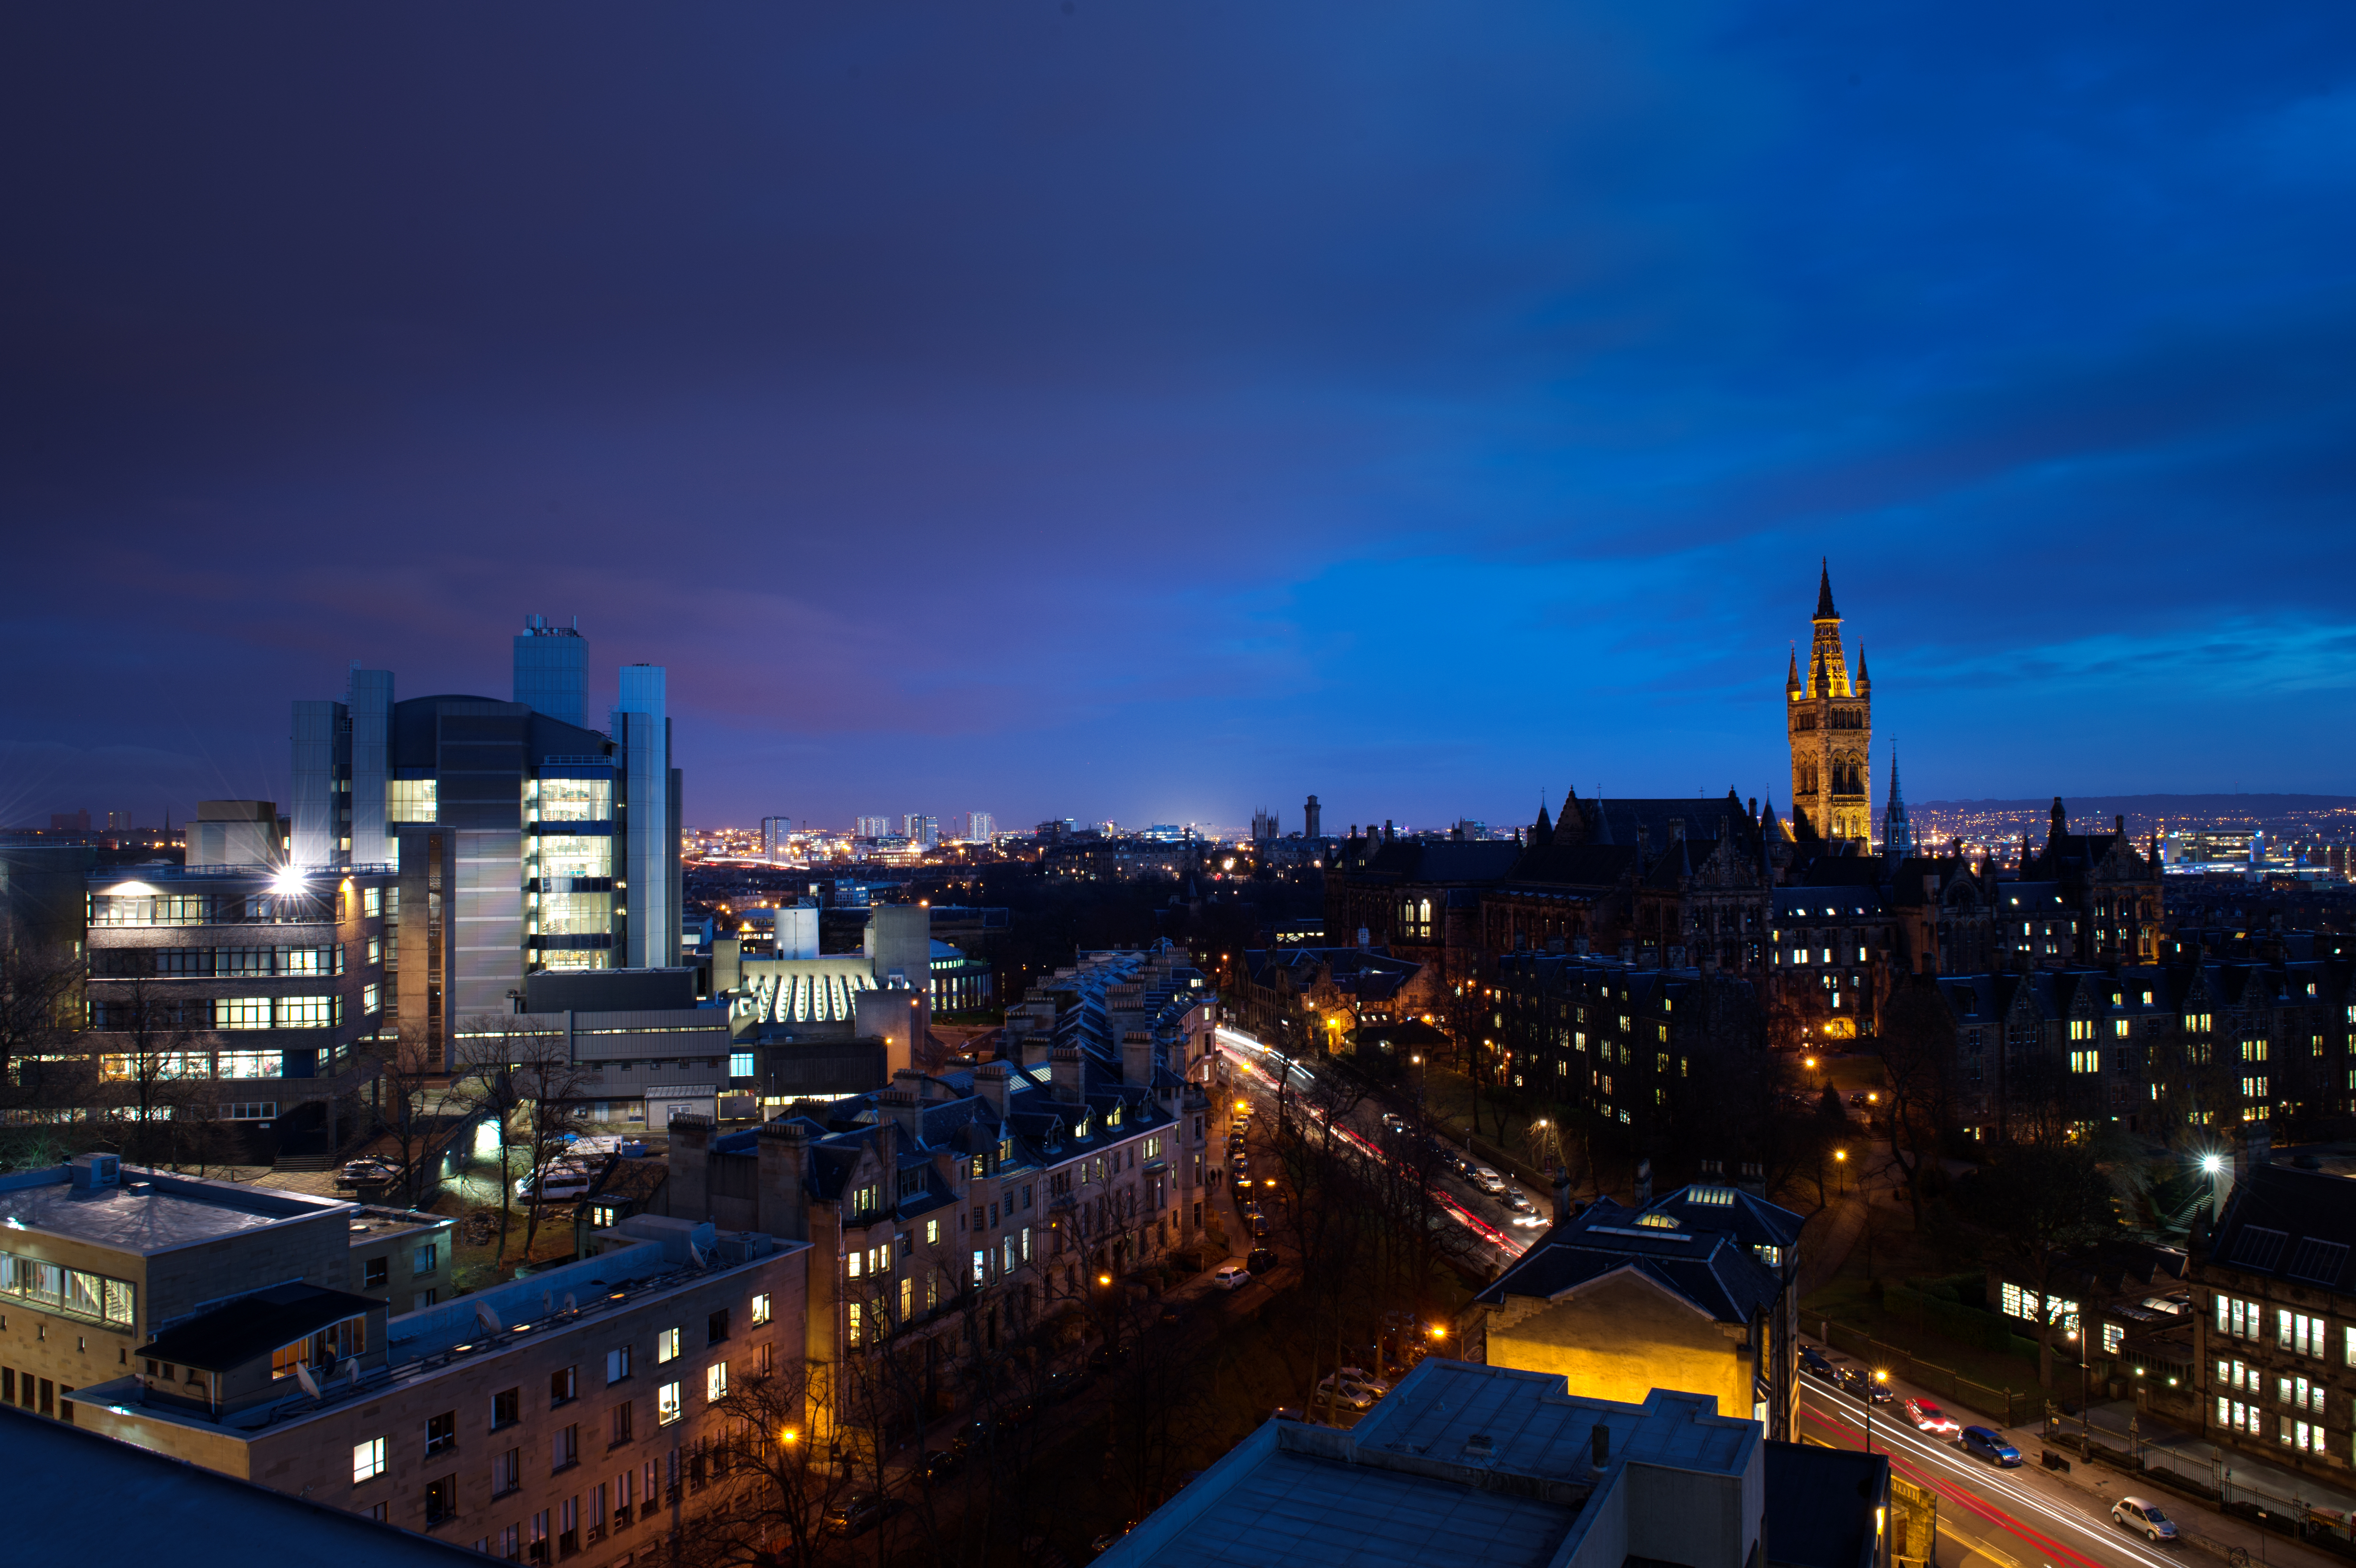
\includegraphics[keepaspectratio=true, width=\paperwidth]{../../images/background2.jpg}};
    }

    \begin{frame}[plain,noframenumbering]
        \begin{tikzpicture}[remember picture, overlay]
            \node at (current page.north west) {
                \begin{tikzpicture}[remember picture, overlay]
                    \fill [fill=uofguniversityblue, anchor=north west] (0, 0) rectangle (\paperwidth, -2.8cm);
                \end{tikzpicture}
            };

            \node (logo) [anchor=north east, shift={(-0.6cm,-0.2cm)}] at (current page.north east) {
                \includegraphics[keepaspectratio=true,scale=0.5]{../../images/UoG_keyline.pdf}
            };

            \node (logo2) [anchor=north, below=0.2cm of logo.south] {
                \includegraphics[keepaspectratio=true,scale=0.1]{../../images/RAEngWhite.pdf}
            };

            \coordinate (logos) at ($(logo.south)!0.5!(logo2.north)$);

            \node [anchor=west, xshift=0.2cm] at (current page.west |- logos) {
                \begin{minipage}{0.60\paperwidth}\raggedright
                    \textcolor{white}{\url{https://ciaranm.github.io/}} \\[0.3cm]
                    \textcolor{white}{\href{mailto:ciaran.mccreesh@glasgow.ac.uk}{\nolinkurl{ciaran.mccreesh@glasgow.ac.uk}}}
                \end{minipage}
            };
        \end{tikzpicture}
    \end{frame}
}

\end{document}

